\section{Testing and Evaluation}
This chapter details testing methodologies used to verify functional and non-functional aspects of the Master Node, IoT Node and the Shipment Tracker Contract.
\subsection{Testing Environment and Strategy}
\vspace{0.5cm}
\subsubsection{Shipment Tracker Contract}
Every function of the Shipment Tracker contract is tested extensively using the Truffle framework and Remix Ethereum IDE. Truffle can be installed using Node Package Manage (NPM). It provides an Ethereum Virtual Machine and a TestRPC client called Ganache CLI. This mimics the Ethereum Network in a sand boxed environment. This client runs on the local machine and simulates the blockchain network. The test RPC client is useful for testing Smart Contracts and decentralized applications before deploying them on the real blockchain.  It makes the process of testing Ethereum Smart Contracts very simple. Ganache CLI is a self-contained private blockchain on a machine. Every transaction sent to this blockchain is immediately mined and confirmed. This allows anyone to quickly test small changes in their contracts.
\vspace{0.5cm}
\subsubsection{Testing Complete System Interaction}
The complete system cannot be tested using the Truffle framework. TestRPC provided by Truffle is a sandboxed blockchain, private to the system where it is running. Individual modules like IoT Node cannot communicate with the private blockchain running on the Master Node. An additional problem is that the blockchain ledger is wiped cleaned when the TestRPC client is closed. The Shipment Tracker Contract is deployed on Ropsten Test Network for testing complete system interactions. Ropsten Test Net closely mimics the main Ethereum blockchain in terms of its operations. Unlike the main blockchain Ropsten Eth can be requested for free from Ropsten faucet \url{https://faucet.ropsten.be/}. This enables anyone to test complete systems without spending money. Transaction confirmation times on Ropsten can vary depending on the network hashing power and load. This makes it unsuitable for module testing or situations where developers need to test small changes quickly.
\vspace{0.5cm}
\subsubsection{Master Node}
Master Node has several components including the GUI, Smart Contract Interface and Raiden Network Interface. The GUI and Raiden Network were tested manually. Raiden token transfers were tested using the Master Node Raiden Module. The token transfers can be validated by calling Raiden API endpoints using command-line tool cURL. The main focus of our testing was the Dapp.js module of the Master Node. This module is used for interacting with the Smart Contract. Two types of testing were performed. TestRPC was used for testing individual functions against locally deployed version of the Shipment Tracker Contract. Full system interaction was also tested by configuring the Master Node to interact with the Shipment Tracker contract, deployed on the Ropsten test network.
\vspace{0.5cm}
\subsubsection{IoT Node}
Ropsten Test Network is used for testing the IoT Node interactions with the Smart Contract. IoT Node was triggered to send violation events to the Shipment Tracker Contract deployed on Ropsten. Validation testing of individual sub modules was performed using Truffle TestRPC. Each major update would go through a suite of validation testing before being deployed on the Raspberry PI. Validation testing was done on a Windows machine. A SensorTest.js class was deployed on the development machines which provided simulated sensor values for development testing. 
\vspace{0.5cm}
\subsection{Testing Scenarios and Results}
This section details various testing scenarios used for validating different system parameters. In order to closely mimic real world use case the Smart Contract was deployed on Ropsten Test Network at the address: \[0x32b1104f718e0c89de5197719e96043f77990c18\]
Unless mentioned otherwise all test cases are using this contract. The contract was deployed using the private key of the Master Node. This gives this node the rights to set requirements, authorize shippers and IoT Nodes and to revoke authorizations.  Data for individual transactions like setting requirements and sending violations etc. can be viewed by using a block explorer. The link to view transaction data is: \url{https://ropsten.etherscan.io/tx/YourTransactionHash}
\vspace{0.5cm}
\subsubsection{Scenario - I}\label{authtesting}
This scenario verifies the behavior of set requirements and authorize shipper functions. This test case will lay the foundation for testing performed in \ref{reqtesting}, \ref{viol1} and \ref{viol2}.

\textbf{Authorization}

Master Node is used for authorizing shippers and IoT Nodes. The hash of the transaction generated as a result of successful call to the authorization function is given below:
\[0x049960bcb0ce5f83289c64b942124c7d7af21a1dd5e2f47fa859fa49cbe7b484\]

We need to verify the following:
\begin{enumerate}
\item Shipper and IoT Node are successfully added to the authorization list.
\item The Smart Contract should fire the AuthorizeAddressEvent. 
\item Only the contract owner is able to authorize shippers and IoT Nodes.
\end{enumerate}

\textbf{Results} 

The list of authorized handlers for any tracking number can be read from the Smart Contract using the Master Node. This verifies that the Shipper and IoT details were successfully added to the blockchain. Master Node detected the AuthorizeAddressEvent event.  The last condition can be verified by calling the authorization function using a different private key then that of the owner. In this case the contract rules will not allow any changes to the contract state. This transaction fails and remaining gas reverted as shown in the figure \ref{fig:AuthorizingHandler}
\vspace{1mm}
\begin{figure}[h]
	\centering
    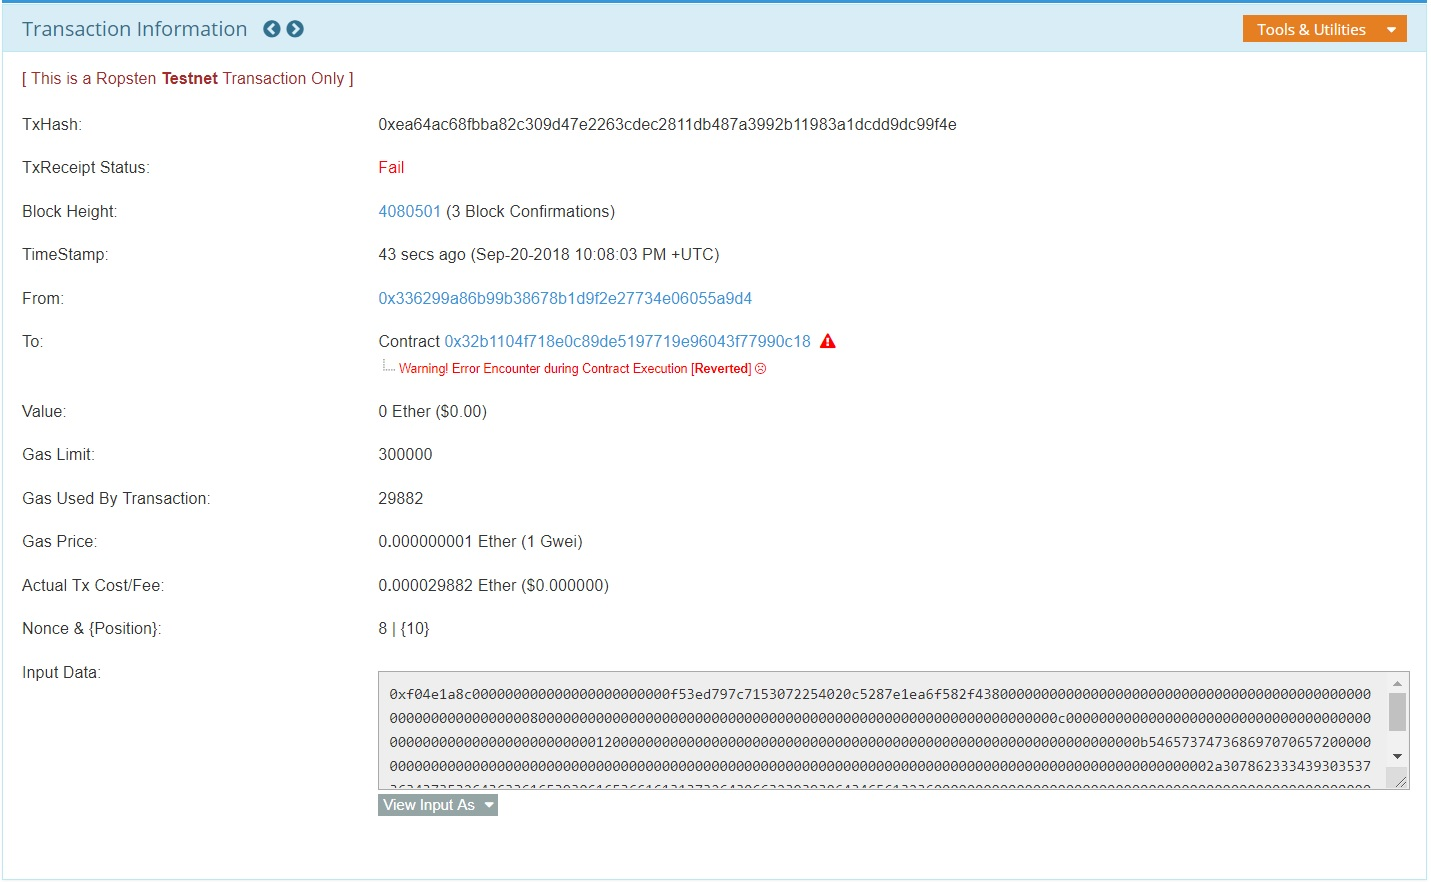
\includegraphics[width=170mm,scale=1]{figs/AuthorizingHandler}
	\caption{Unauthorized modifications of the handler list are not allowed}
	\label{fig:AuthorizingHandler} 
\end{figure}

\clearpage
%\vspace{0.5cm}
\subsubsection{Scenario - II} \label{reqtesting} 
\textbf{Testing Requirements}

This scenario validates the requirement feature of our system. Requirements are set for a specific package or supply line. The tracking number for the test package will be “TestCase001”. Master Node is used to set a requirement with the requirement ID ‘LUX’ as shown in the figure \ref{fig:SetRequirements}. The maximum threshold value is set to 200. Max flag is set. This indicates to the IoT Node that only maximum threshold is of interest for this requirement.

\begin{figure}[!h]
	\centering
    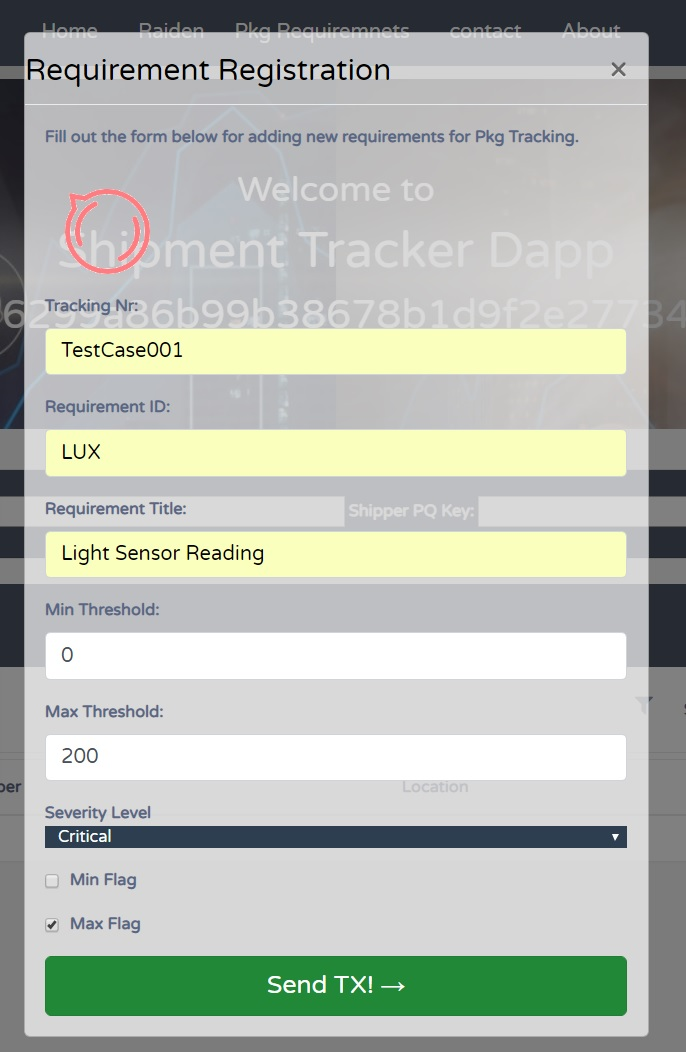
\includegraphics[width=100mm,scale=1]{figs/SetRequirements}
	\caption{Setting light sensor requirement}
	\label{fig:SetRequirements} 
\end{figure}

The transaction hash for the successful transaction is given below:
\[0x589b96de8e100519fcbcd481dd8b54d02a314a68e70ab2aa29d75143d712c4fc\]

We need to verify the following:

\begin{enumerate}
\item Requirements are successfully added to the requirement list in the blockchain.
\item Requirement event is fired from the Shipment Tracker Contract. 
\item Only the contract owner should be able to define requirements.
\item A correctly initialized and authorized IoT Node can read requirements from the blockchain.
\item  IoT Node initializes the correct sensor (light sensor) and starts the logging process.
\end{enumerate}

\textbf{Results}

The transaction for requirement ID LUX is successful. This requirement is successfully saved in the blockchain. The Master Node detects the new requirement event. The transaction generated using a different Ethereum key fails. This verifies that only contract owner is allowed to set requirements.
 
\textbf{IoT Node:}
The IoT node is initialized with the tracking number “TestCase001”. This node was authorized to read requirements for this tracking number in \ref{authtesting}. The Requirement ID corresponds to the Light Sensor in the IoT node. The IoT Node successfully reads the requirements and starts the monitoring process as show in figure \ref{fig:IoTreq}.

\begin{figure}[h]
	\centering
    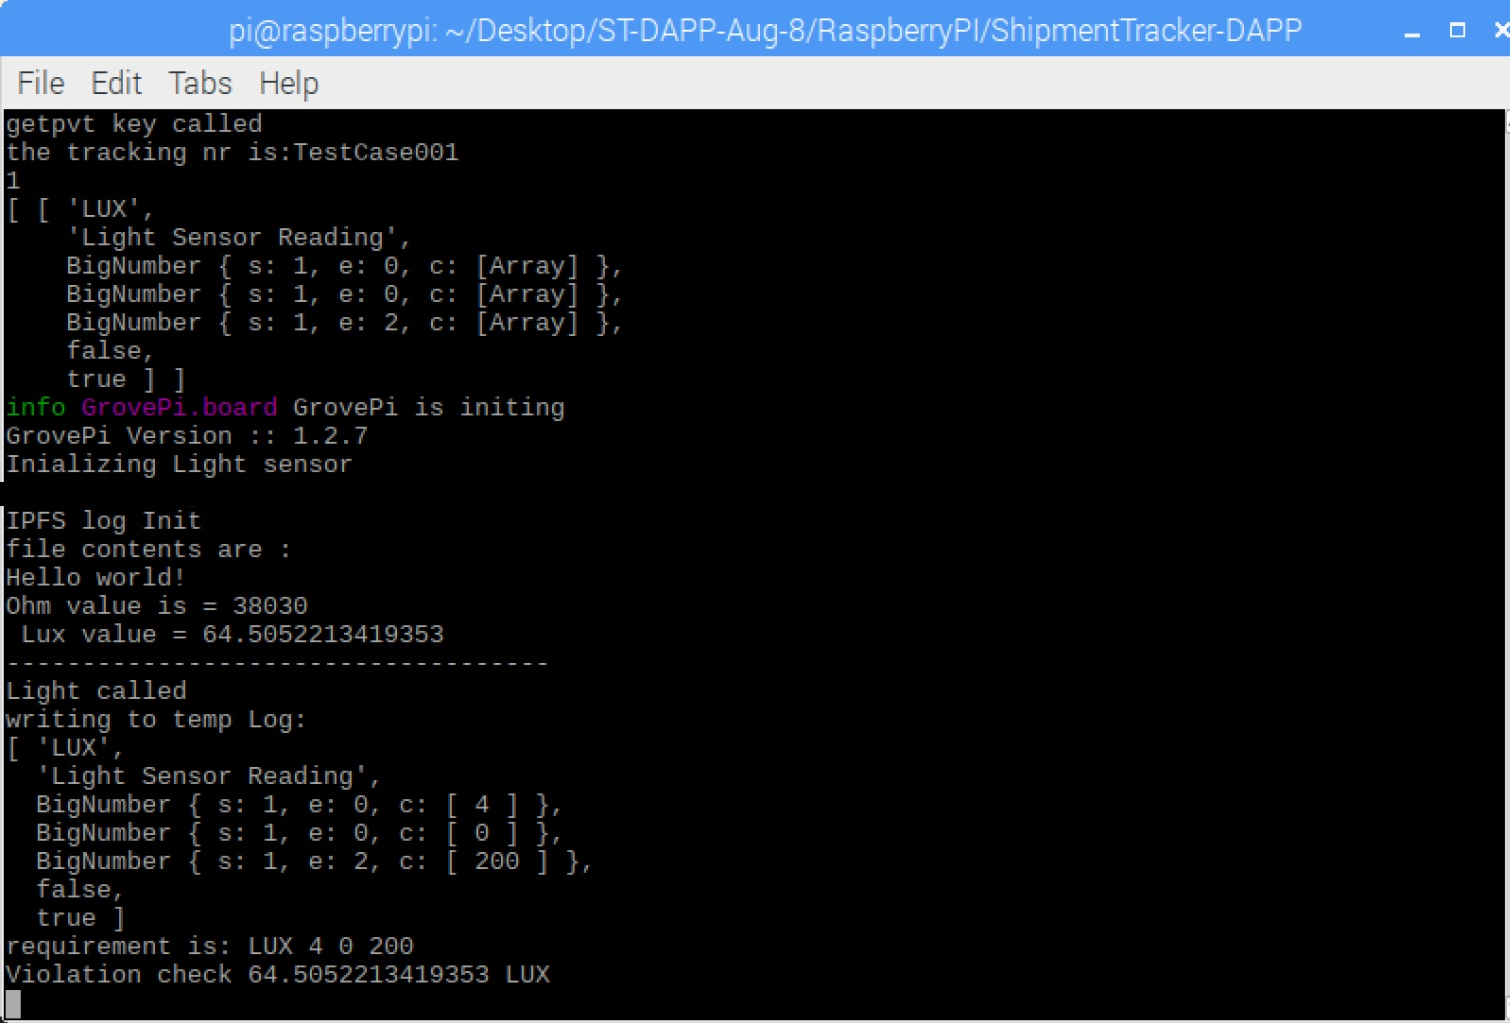
\includegraphics[width=140mm,scale=1]{figs/IoTreq}
	\caption{IoT Node reading requirements}
	\label{fig:IoTreq} 
\end{figure}

\subsubsection{Scenario - III}
This test case models a simple scenario involving a single shipper and no violations. One shipper is responsible for delivering the package from the  supplier warehouse to the factory floor. The IoT Node monitors package exposure to temperature (Temp), light (LUX) and pressure (PRESSURE). In this case only two transactions are saved in the blockchain. One to indicate delivery of the package, second to save the IPFS hash of the log file at the end of the delivery cycle. The monitoring interval is set to 1 minute. This scenario verifies the following:
 \begin{enumerate}
\item Multiple requirements are successfully monitored by the IoT Node.
\item Detailed log is saved in IPFS. 
\item IPFS log hash is successfully saved in the Shipment Tracker Contract.
\end{enumerate}

\textbf{Results}

The IPFS log address is automatically saved to the Shipment Tracker Contract when the package status changes from shipping to delivered. The shipping status can be manually changed to delivered or it can change in response to an external event. This could be a scan event at the factory floor. Alternatively, IoT Node can be programmed to change the shipping status automatically based on location data received from the GPS sensor. Figure \ref{fig:IPFSlog} shows the monitoring log generated for this test case.

\begin{figure}[h]
	\centering
    \includegraphics[width=170mm,scale=1]{figs/IPFSlog}
	\caption{Monitoring log saved on IPFS}
	\label{fig:IPFSlog} 
\end{figure}


The IPFS address for this log is given below
\[QmPDT5VnQ6m57XTgskjdSHPrMZotd6hGaakv8JQca7tCMN\]




\subsubsection{Scenario - IV} \label{viol1} 
This test case models the scenario with multiple shippers and multiple violations. The package number “TestCase001” is monitoring temperature, light and humidity. There are three shippers involved in shipping cycle. The shipper change event can be simulated using a push button. A test class detects the button press events, and sends the new shipper ID and PQ key to the IoT Node.  Three shippers, namely “DHLShipper1”, “DHLShipper2”, and “PostShipper2”, were authorized to handle the package. In actual scenarios package handover event (shipper change) will be detected using an NFC chip.  Master Node and Shippers can subscribe to violation events to get real time information about package conditions.

\textbf{Results}

There were two violation events detected, a temperature violation and a light violation. The temperature violation was simulated using human body heat on the sensor. The maximum temperature threshold was set to 30 degrees Celsius. The light violation was simulated by exposing the light sensor to direct sunlight. Master Node was able to detect the violation events fired from the Shipment Tracker Contract. Master Node can be used to determine which shipper was responsible for the violation. An example of this is shown in \ref{fig:violationEvent}.
 
\begin{figure}[h]
	\centering
    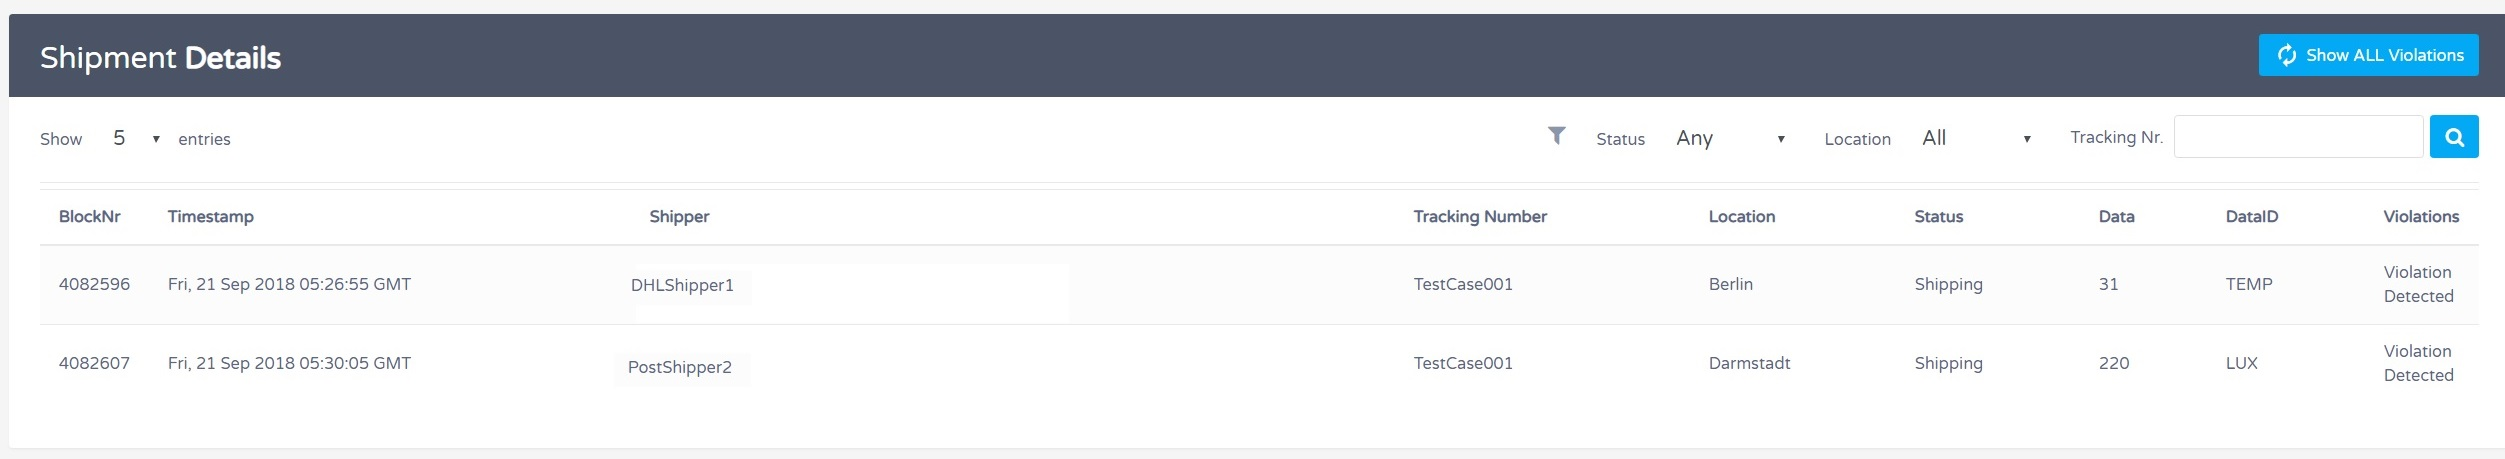
\includegraphics[width=170mm,scale=1]{figs/violationEvent}
	\caption{Master Node detects violations}
	\label{fig:violationEvent} 
\end{figure}


Violation transactions are sent from the IoT Node to the Smart Contract. Smart Contract verfies that the transaction is reporting a legitimate violation. If violations are confirmed the Smart Contract fires appropriate violation events. The hashes for the two transactions are given below: %The first transaction reported temperature max threshold violation. Second transaction reported exposure to high intensity light. Shipment Tracker contract fired the relevant violation events for both cases.

Temperature violation: 
\[ 0xc0d85edc38b955055e6a203c3d5c5b400e4324d47a467431b590e71f501ebab2\]
Light Violation: \[0x9b1758c50663f386c334838b1861cccd96e03f20bb62dd6160cca3cbcff3a068\]


\subsubsection{Scenario - V} \label{viol2} 
This test case models the scenario of an organization having multiple concurrent supply lines with different shippers and suppliers. This is the realistic case in many medium or large organization operating a Just-in-Time- Supply chain. This experiment focuses on the performance of the Shipment Tracker Contract under sustained load of multiple violations sent from different supply lines. 

\textbf{Test Setup}

A test program is written to simulate an IoT Node sending shipping violations to the Smart Contract. Four supply lines, namely “TestCase001”, “TestCase002”, “TestCase003” and “TestCase004”, are defined. Each supply line has two to three authorized handlers. The test program is executed on three machines. Each machine ran up to four instances of this program for a total of up to twelve concurrent shippers. Each shipper sent violations after an interval of 1 to 2 minutes. Etherscan is used to determine average transaction confirmation time. It is also used to determine when a violation event is fired from the Smart Contract. Master Node logs the time when it receives shipping violation events.

\textbf{Results}

The results of this experiment are summarized in table \ref{table:t21}. The Event Latency defines the interval between the Shipment Tracker firing an event till it is seen at the Master Node. This experiment indicates that event latency is not effected by transaction load and is largely due to transport and network delays. This table shows that in the best case scenario the number of concurrent shippers do not affect the system performance or transaction confirmation times. There are certain scenarios where system performance will be affected (see scaling debate \ref{scaling}). These include factors such as a drop in network hash power or an adverse and exponential increase in network load i.e. number of overall transactions sent to the blockchain. These factors are beyond our control and are effecting the blockchain community as a whole. Developers are working on proposals for scaling public blockchains as discussed in \ref{scaling}. Alternatively, a private or consortium blockchain such as Hyperledger Fabric can be used to mitigate some of these factors.     
\vspace{1mm}
\begin{table}[h]
\centering
\resizebox{\columnwidth}{!}{
\begin{tabular}{|c|c|c|c|}
\hline
\rowcolor[HTML]{5B82BA} 
{\color[HTML]{FFFFFF} \textbf{Nr. of Concurrent Shippers}} & {\color[HTML]{FFFFFF} \textbf{Avg. Confirmation Time}} & {\color[HTML]{FFFFFF} \textbf{Avg. Transaction Cost}} & {\color[HTML]{FFFFFF} \textbf{Event Latency}} \\ \hline
1                                                          & 1 - 2 mins                                             & 0.10 \$                                               & \textless 1 sec                               \\ \hline
3                                                          & 1 - 2 mins                                             & 0.10\$                                                & \textless 1 sec                               \\ \hline
6                                                          & 1 - 2 mins                                             & 0.10\$                                                & \textless 1 sec                               \\ \hline
9                                                          & 1 - 2 mins                                             & 0.10\$                                                & \textless 1 sec                               \\ \hline
12                                                         & 1 - 2 mins                                             & 0.10\$                                                & \textless 1 sec                               \\ \hline
\end{tabular}
}
\caption {Performance Impact of Multiple Concurrent Shippers on Decentralized Shipment Tracker}
\label{table:t21}
\end{table}



\subsection{Evaluation}
The evaluations presented in this section are based on approximations using volatile data like Eth price and Gas Price. The volatile nature of these key transaction parameters make it difficult to perform accurate estimations.

\textbf{Tools Used:} \url{https://etherscan.io/}, \url{https://ethgasstation.info/}
\vspace{0.5cm}
\subsubsection{Transaction Speed and Cost} \label{TrxCost} 
Section \ref{trxprice} showed that the total transaction cost can be calculated by multiplying the gas used by the transaction with the gas price. The user is allowed to set the gas price for individual transactions. This price usually determines how fast on average the transaction will be confirmed. Miners usually prefer transactions with higher gas prices over others. If the price is too low, miners will simply ignore the transaction. Minimum safe gas price can be found using \url{https://ethgasstation.info/}. This price depends upon network conditions like transaction load and hashing power. The table \ref{table:t2} given below shows gas prices as observed on two different dates. The total gas required by a transaction depends on the type of operation it will perform and will largely remain constant for the same type of transactions.
\vspace{1mm}
\begin{table}[h]
\centering
%\resizebox{\columnwidth}{!}{%
\begin{tabular}{|c|c|c|}
\hline
\rowcolor[HTML]{5B82BA} 
\multicolumn{1}{|l|}{\cellcolor[HTML]{5B82BA}{\color[HTML]{FFFFFF} \textbf{Date}}} & {\color[HTML]{EFEFEF} \textbf{Speed}} & {\color[HTML]{EFEFEF} \textbf{Gas Price (gwei)}} \\ \hline
                                                                                   & SafeLow (\textless{}30m)              & 3                                                \\ \cline{2-3} 
                                                                                   & Standard (\textless{}5m)              & 5                                                \\ \cline{2-3} 
\multirow{-3}{*}{16 September 2018}                                       & Fast (\textless{}2m)                  & 6                                                \\ \hline
                                                                                   & SafeLow(\textless{}30m)               & 25                                               \\ \cline{2-3} 
                                                                                   & Standard(\textless{}5m)               & 45                                               \\ \cline{2-3} 
\multirow{-3}{*}{4 December 2017}                                         & Fast(\textless{}2m)                   & 57                                               \\ \hline
\end{tabular}%
%}
\caption {Gas Price and transaction times}
\label{table:t2}
\end{table}
\vspace{0.5cm}
\subsubsection{Contract Deployment Cost}
Initial architecture design called for using separate Smart Contracts for individual shipping cycles. The idea was a new contract would be deployed at the start of each shipping cycle. However, it was quickly realized this would lead to segregation of information. This would also be expensive in terms of operations, deployment and maintenance, specially on a public blockchain like Ethereum. Figure \ref{fig:STC} shows the transaction for deploying the Shipment Tracker Contract using MetaMask. 
\clearpage
\begin{figure}[!h]
	\centering
    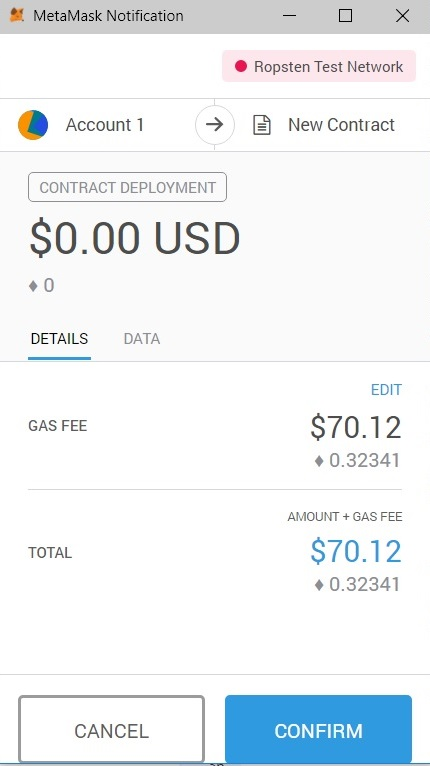
\includegraphics[width=60mm,scale=0.5]{figs/STC}
	\caption{Deploying Shipment Tracker contract using MetaMask}
	\label{fig:STC} 
\end{figure} 

Table \ref{table:t3} shows cost of deploying Shipment Tracker and Helper Contracts. Eth prices on two different dates were taken into account to elaborate the worst case and average case scenarios. Ethereum prices can fluctuate by significant amounts from one day to another. Contract deployment is one of the most expensive transaction in any Ethereum based system. Considering this and other factors listed above, It was decided to design a contract that could handle multiple shipping cycles in parallel. This contract is more complex and hence costs more to deploy compared to contracts that would handle only one shipping cycle. However, this contract is deployed once and is designed to be much more efficient in terms of operations and maintenance.
\vspace{1mm}
\begin{table}[h]
\centering
\resizebox{\columnwidth}{!}{%
\begin{tabular}{|l|l|l|l|c|}
\hline
\rowcolor[HTML]{5B82BA} 
\multicolumn{1}{|c|}{\cellcolor[HTML]{5B82BA}{\color[HTML]{FFFFFF} \textbf{Contract}}} & \multicolumn{1}{c|}{\cellcolor[HTML]{5B82BA}{\color[HTML]{FFFFFF} \textbf{Gas Limit}}} & \multicolumn{1}{c|}{\cellcolor[HTML]{5B82BA}{\color[HTML]{FFFFFF} \textbf{Deployment Cost}}} & \multicolumn{1}{c|}{\cellcolor[HTML]{5B82BA}{\color[HTML]{FFFFFF} \textbf{Gas Price}}} & {\color[HTML]{FFFFFF} \textbf{Price of 1 ETH}} \\ \hline
Helper.sol                                                                    & 922416 gwei                                                                            & 10\$                                                                                         &                                                                                        &                                                \\ \cline{1-3}
ShipmentTracker.sol                                                           & 6468201 gwei                                                                           & 70.2\$                                                                                       & \multirow{-2}{*}{15 gwei}                                                              & \multirow{-2}{*}{222\$}                        \\ \hline
Helper.sol                                                                    & 922416 gwei                                                                            & 116.4\$                                                                                      &                                                                                        &                                                \\ \cline{1-3}
ShipmentTracker.sol                                                           & 6468201 gwei                                                                           & 388.092\$                                                                                    & \multirow{-2}{*}{55 gwei}                                                              & \multirow{-2}{*}{1200\$}                       \\ \hline
\end{tabular}%
}
\caption {Cost of Contract Deployment}
\label{table:t3}
\end{table}

\clearpage
\subsubsection{Cost of Storage on the Blockchain}
In section \ref{IPFS} it was mentioned that it is prohibitively expensive to store large chunks of data on the blockchain. Table \ref{table:t4} shows the cost of storage on the Ethereum blockchain. In this scenario the minimum observed Eth price was used for calculations. Log size in our system depends on the log interval and number of attached sensors. In an actual use case scenario an organization would want to keep in depth logs of each and every activity. This would lead to a large log files for each shipping cycle.  This table makes it obvious that it is not feasible to store logging information in the blockchain. In depth logs are stored using IPFS. If the log interval is set to five minutes a 1KB log file is generated after one hour. IPFS allows the flexibility to make the log interval as small as required. 
\vspace{1mm}
\begin{table}[h]
\centering
\resizebox{\columnwidth}{!}{%
\begin{tabular}{|c|c|c|c|c|}
\hline
\rowcolor[HTML]{5B82BA} 
{\color[HTML]{FFFFFF} \textbf{Data size}} & {\color[HTML]{FFFFFF} \textbf{Gas Required}} & {\color[HTML]{FFFFFF} \textbf{\begin{tabular}[c]{@{}c@{}}Transaction Cost\\ (Eth)\end{tabular}}} & {\color[HTML]{FFFFFF} \textbf{ETH  Price}} & \multicolumn{1}{l|}{\cellcolor[HTML]{5B82BA}{\color[HTML]{FFFFFF} \textbf{\begin{tabular}[c]{@{}l@{}}Cost of Storage\\ (Eth*Eth Price)\end{tabular}}}} \\ \hline
256 bit word                              & 20000                                        & 0.0006                                                                                           &                                            & 0.133\$                                                                                                                                                \\ \cline{1-3} \cline{5-5} 
1MB                                       & 625 Million                                  & 18.75                                                                                            &                                            & 4162\$                                                                                                                                                 \\ \cline{1-3} \cline{5-5} 
10MB                                      & 6.25 Billion                                 & 187.5                                                                                            &                                            & 41,625\$                                                                                                                                               \\ \cline{1-3} \cline{5-5} 
100MB                                     & 62 Billion                                   & 1875                                                                                             & \multirow{-4}{*}{222\$}                    & 116,250\$                                                                                                                                              \\ \hline
\end{tabular}
}
\caption {Cost of Storage on Ethereum Blockchain}
\label{table:t4}
\end{table}
\vspace{0.5cm}
\subsubsection{Cost of storing Violations and Requirements}
Operational costs depend upon transaction costs for storing violations and defining requirements. Both transactions use almost equivalent amount of gas. The calculations shown in table \ref{table:t4} are based on a transaction generated for defining temperature requirement. The gas price for this transaction was set to 20 gwei. It spent 0.00484134 Eth worth of gas. This is equivalent to 1 dollar according to the Eth pricing as of 17 August 2018. Alternatively, when Eth pricing from January 2018 are taken into account, the cost of this transaction becomes 5 dollars. The table \ref{table:t4} given below shows daily operational cost based on best case and worst case scenarios. The worst case simulates violations issued for four sensors attached to the IoT Node. In this case each type of violation is stored once, and repeated violations of the same type will be stored in IPFS. The worst case simulates a large organization with multiple suppliers and multiple shipments on route at the same time. The table calculations are based on five parallel supply lines.
%\vspace{1mm}
\begin{table}[h]
\centering
\resizebox{\columnwidth}{!}{%
\begin{tabular}{|c|c|c|c|c|c|c|}
\hline
\rowcolor[HTML]{5B82BA} 
{\color[HTML]{FFFFFF} \textbf{}} & {\color[HTML]{FFFFFF} \textbf{Number of Violations}} & {\color[HTML]{FFFFFF} \textbf{Transaction Cost}} & {\color[HTML]{FFFFFF} \textbf{Gas Price}} & {\color[HTML]{FFFFFF} \textbf{Price of 1 ETH}} & \multicolumn{1}{l|}{\cellcolor[HTML]{5B82BA}{\color[HTML]{FFFFFF} \textbf{Number of Supply lines}}} & \multicolumn{1}{l|}{\cellcolor[HTML]{5B82BA}{\color[HTML]{FFFFFF} \textbf{Daily Cost}}} \\ \hline
\textbf{Best Case}               & 0                                                    & 0\$                                              &                                           &                                                & 1                                                                                                   & 0\$                                                                                     \\ \cline{1-3} \cline{6-7} 
\textbf{Worst Case}              & 4                                                    & 1\$                                              & \multirow{-2}{*}{20 gwei}                 & \multirow{-2}{*}{222\$}                        & \textgreater{}5                                                                                     & 20\$                                                                                    \\ \hline
\textbf{Best Case}               & 0                                                    & 0\$                                              &                                           &                                                & 1                                                                                                   & 0                                                                                       \\ \cline{1-3} \cline{6-7} 
\textbf{Worst Case}              & 4                                                    & 4\$                                              & \multirow{-2}{*}{20 gwei}                 & \multirow{-2}{*}{1200\$}                       & \textgreater{}5                                                                                     & 80\$                                                                                    \\ \hline
\end{tabular}%
}
\label{table:t5}
\caption{Daily Operational Cost}
\end{table}
